\begin{figure}[t]
  \centering
  \subfloat[SH]{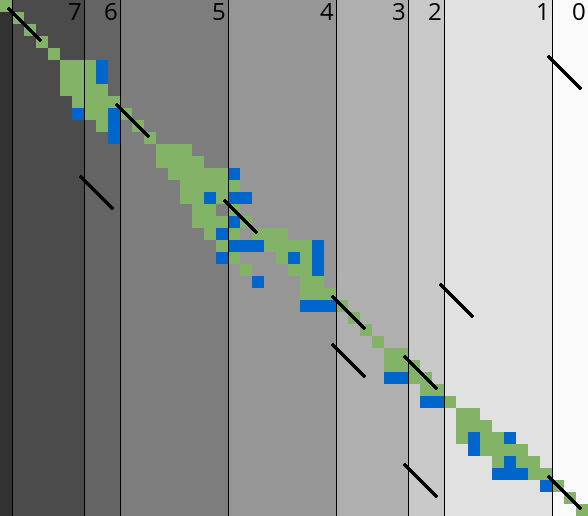
\includegraphics[width=0.32\linewidth]{imgs/layers/sh-noprune.png}\label{fig:layers-sh}}
  \hfill
  \subfloat[CSH]{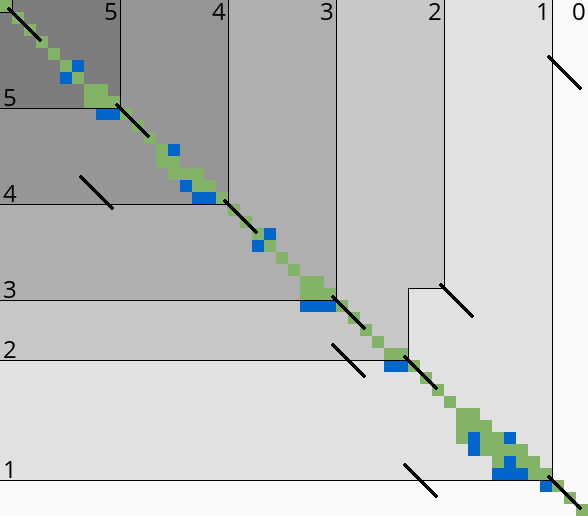
\includegraphics[width=0.32\linewidth]{imgs/layers/csh-noprune.png}\label{fig:layers-csh}}
  \hfill
  \subfloat[\GCH]{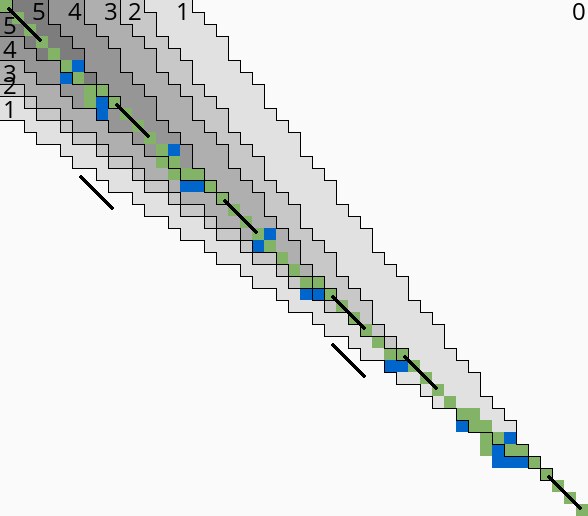
\includegraphics[width=0.32\linewidth]{imgs/layers/gcsh-noprune.png}\label{fig:layers-gcsh}}
  \\
  \subfloat[SH + pruning]{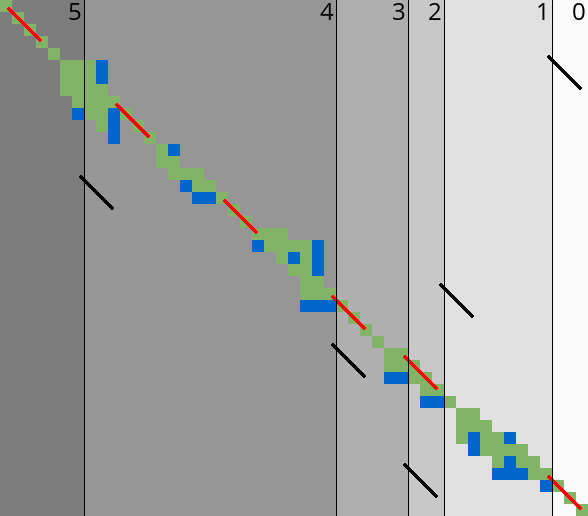
\includegraphics[width=0.32\linewidth]{imgs/layers/sh.png}\label{fig:layers-sh-pruning}}
  \hfill
  \subfloat[CSH + pruning]{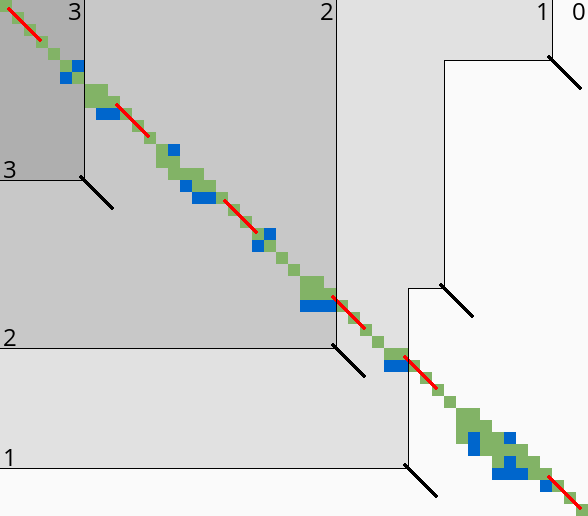
\includegraphics[width=0.32\linewidth]{imgs/layers/csh.png}\label{fig:layers-csh-pruning}}
  \hfill
  \subfloat[\GCH +
  pruning]{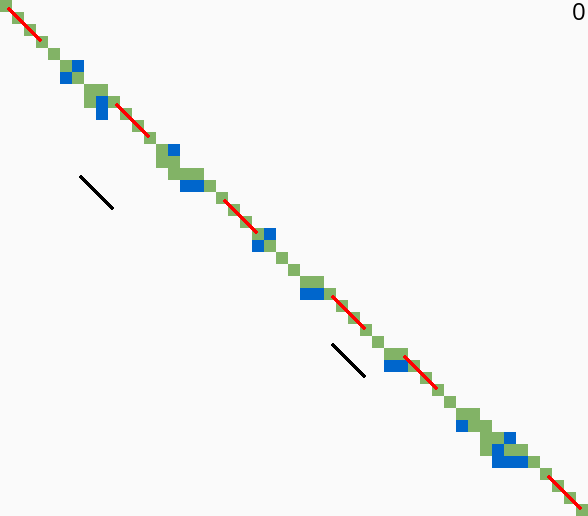
\includegraphics[width=0.32\linewidth]{imgs/layers/gcsh.png}\label{fig:layers-gcsh-pruning}}
  \caption[Contours and layers of different seed heuristics]{\textbf{Contours and layers of different heuristics after aligning}
  ($n{=}48$, $m{=}42$, $r{=}1$, $k{=}3$, edit distance $10$). Exact matches are
  black diagonal segments~(\blackmatch{}). The background colour indicates
  $S_p(u)$, the maximum number of matches on a $\preceq_p$-chain from $u$ to the
  end starting, with $S_p(u) = 0$ in white. The thin black boundaries of these
  regions are \emph{Contours}. The states of layer $\layer_\ell$ \emph{precede}
  contour $\ell$. Expanded states are green~(\greensquare{}), open states
  blue~(\bluesquare{}), and pruned matches red~(\redmatch{}). Pruning matches
  changes the contours and layers. \GCH ignores matches $m{\npreceq_T}v_t$.}
  \label{fig:contours}
\end{figure}
